\section{Integral of the Gaussian bell curve} \label{sec:gauss_general}
The shifted Gaussian bell function, shown in the figure \ref{fig:tikz_gauss_curve_general}, is used to model the solar energy curve (see subsection \ref{sec:solar_energy_curve}). Therefore, the mathematical approach of calculating the area of the Gaussian bell function -- enclosed by the curve and the x-axis -- will be explained.
\begin{figure}[h!]
	\centering
	
\tikzset{every picture/.style={line width=0.75pt}} %set default line width to 0.75pt        

\begin{tikzpicture}[x=0.75pt,y=0.75pt,yscale=-1,xscale=1]
%uncomment if require: \path (0,300); %set diagram left start at 0, and has height of 300

%Image [id:dp36698085633645405] 
\draw (328.75,179) node  {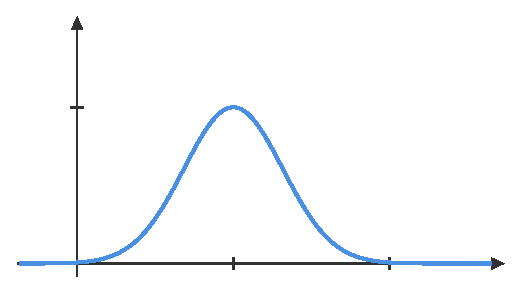
\includegraphics[width=233.63pt,height=124.5pt]{images/image_shifted_gauss_curve}};
%Straight Lines [id:da37857254246955074] 
\draw [color={rgb, 255:red, 155; green, 155; blue, 155 }  ,draw opacity=1 ] [dash pattern={on 4.5pt off 4.5pt}]  (222,153.7) -- (303.4,153.7) ;
%Straight Lines [id:da32947142925776296] 
\draw [color={rgb, 255:red, 155; green, 155; blue, 155 }  ,draw opacity=1 ] [dash pattern={on 4.5pt off 4.5pt}]  (311.4,243) -- (311.4,155.7) ;
%Shape: Circle [id:dp5744124003855682] 
\draw  [fill={rgb, 255:red, 255; green, 255; blue, 255 }  ,fill opacity=1 ] (309.4,153.7) .. controls (309.4,152.6) and (310.3,151.7) .. (311.4,151.7) .. controls (312.5,151.7) and (313.4,152.6) .. (313.4,153.7) .. controls (313.4,154.8) and (312.5,155.7) .. (311.4,155.7) .. controls (310.3,155.7) and (309.4,154.8) .. (309.4,153.7) -- cycle ;

% Text Node
\draw (202.5,76.9) node [anchor=north west][inner sep=0.75pt]  [font=\footnotesize]  {$f( x)$};
% Text Node
\draw (488,248.4) node [anchor=north west][inner sep=0.75pt]  [font=\footnotesize]  {$x$};
% Text Node
\draw (305,262.9) node [anchor=north west][inner sep=0.75pt]  [font=\footnotesize]  {$x_{0}$};
% Text Node
\draw (397.5,259.4) node [anchor=north west][inner sep=0.75pt]  [font=\footnotesize]  {$2x_{0}$};
% Text Node
\draw (197,256.4) node [anchor=north west][inner sep=0.75pt]  [font=\footnotesize]  {$0$};
% Text Node
\draw (191,147.4) node [anchor=north west][inner sep=0.75pt]  [font=\footnotesize]  {$C$};


\end{tikzpicture}


	\caption{Shifted Gauss bell.}
	\label{fig:tikz_gauss_curve_general}
\end{figure}

In general, the Gaussian bell function can be written as shown in the equation (\ref{eq:gauss_curve}), with its corresponding indefinite Integral shown in the equation (\ref{eq:integral_gauss}).
\begin{center}
	\begin{equation} \label{eq:gauss_curve}
		f\left(x\right) = C \, \exp\left(-\frac{(x - x_0)^2}{a}\right)
	\end{equation}
\end{center}
\begin{center}
	\begin{equation} \label{eq:integral_gauss}
		F\left(x\right) = C \int\limits_{-\infty}^{\infty} \exp\left(-\frac{(x - x_0)^2}{a}\right)\,\mathrm{d}x
	\end{equation}
\end{center}
Since the integral in the equation (\ref{eq:integral_gauss}) cannot be solved, an approach is used in which the integral is squared. How this works is presented in the following steps.
\begin{center}
	\begin{equation} \label{eq:integral_gauss_partly_solved}
		\begin{aligned}
		F\left(x\right)^2 &= C^2 \left( \, \int\limits_{-\infty}^{\infty} \exp\left(-\frac{(x - x_0)^2}{a}\right)\,\mathrm{d}x\right)^2 \\
		&= C^2 \int\limits_{-\infty}^{\infty} \exp\left(-\frac{(u - u_0)^2}{a}\right)\,\mathrm{d}u \int\limits_{-\infty}^{\infty} \exp\left(-\frac{(v - v_0)^2}{a}\right)\,\mathrm{d}v \\ 
		&= C^2 \int\limits_{-\infty}^{\infty} \int\limits_{-\infty}^{\infty} \exp\left(-\frac{(u - u_0)^2}{a}\right) \, \exp\left(-\frac{(v - v_0)^2}{a}\right) \,\mathrm{d}u \cdot \mathrm{d}v \\
		&= C^2 \int\limits_{-\infty}^{\infty} \int\limits_{-\infty}^{\infty} \exp\left(-\frac{(u - u_0)^2 + (v - v_0)^2}{a}\right) \,\mathrm{d}u \cdot \mathrm{d}v
		\end{aligned}
	\end{equation}
\end{center}
If now $x = u - u_0$ and $y = v - v_0$ are substituted in the last step of the equation (\ref{eq:integral_gauss_partly_solved}), the double integral can be written as presented in the equation (\ref{eq:integral_gauss_not_shifted}). Due to these substitutions, the equations (\ref{eq:diff}) to (\ref{eq:lim_y}) have to be considered. 
\begin{center}
	\begin{equation} \label{eq:diff}
		\mathrm{d}x = \mathrm{d}u \text{, } \mathrm{d}y = \mathrm{d}v
	\end{equation}
\end{center}
\begin{center}
	\begin{equation} \label{eq:lim_x}
		\lim\limits_{u \to \infty} x = \infty \text{, } \lim\limits_{u \to -\infty} x = -\infty
	\end{equation}
\end{center}
\begin{center}
	\begin{equation} \label{eq:lim_y}
		\lim\limits_{v \to \infty} y = \infty \text{, } \lim\limits_{v \to -\infty} y = -\infty
	\end{equation}
\end{center}
By using the expressions from the equation (\ref{eq:polar}), the double integral in the equation (\ref{eq:integral_gauss_not_shifted}) can be transformed into polar coordinates.
\begin{center}
	\begin{equation} \label{eq:polar}
		x^2 + y^2 = r^2 \text{, } \mathrm{d}x \, \mathrm{d}y = r \, \mathrm{d}r \,\mathrm{d}\phi
	\end{equation}
\end{center}
\begin{center}
	\begin{equation} \label{eq:integral_gauss_not_shifted}
		\begin{aligned}
		F\left(x\right)^2 &= C^2 \int\limits_{-\infty}^{\infty} \int\limits_{-\infty}^{\infty} \exp\left(-\frac{x^2 + y^2}{a}\right) \,\mathrm{d}x \cdot \mathrm{d}y \\
		&= C^2 \int\limits_{0}^{2\pi} \int\limits_{0}^{\infty} \exp\left(-\frac{r^2}{a}\right) \, r \,\mathrm{d}r \cdot \mathrm{d}\phi
		\end{aligned}
	\end{equation}
\end{center}
With a final substitution of $w = -\frac{r^2}{a}$, from which the equations (\ref{eq:diff_r}) and (\ref{eq:lim_r}) derive, the double integral can be solved as shown in the equation (\ref{eq:integral_gauss_solved}).
\begin{center}
	\begin{equation} \label{eq:diff_r}
		r\,\mathrm{d}r = -\frac{a}{2} \, \mathrm{d}u
	\end{equation}
\end{center}
\begin{center}
	\begin{equation} \label{eq:lim_r}
		\lim\limits_{r \to \infty} w = -\infty \text{, } \lim\limits_{r \to 0} w = 0
	\end{equation}
\end{center}
\begin{center}
	\begin{equation} \label{eq:integral_gauss_solved}
		\begin{split}
		F\left(x\right)^2 = -\frac{a \, C^2}{2}\int\limits_{0}^{2\pi} \underbrace{\int\limits_{0}^{-\infty} \mathrm{e}^w \,\mathrm{d}w}_{-1} \cdot \mathrm{d}\phi = \frac{a \, C^2}{2}\int\limits_{0}^{2\pi} 1 \, \mathrm{d}\phi = a \, C^2 \, \pi
		\end{split}
	\end{equation}
\end{center}
The result of the indefinite integral of the Gaussian bell function must therefore be:
\begin{center}
	\begin{equation} \label{eq:result}
		F(x) = C \sqrt{a \, \pi} \text{.}
	\end{equation}
\end{center}
It is positive because the area enclosed by the curve and the x-axis cannot be negative. 
